\section{Objets DICOM}

\frame
{
 	\frametitle{Information Object Definition}
  	L'IOD d�termine les attributs d�crivant un objet.
  	\begin{description}
    	\item[Normalized IOD] Repr�sente une entit� unique du monde r�el (patient, visite, examen, r�sultat, interpr�tation,?).
		Rarement appliqu� en pratique : cause complexit� et perte de performance.
    	\item[Composite IOD] Repr�sente certains d�tails de plusieurs objets du monde r�el et les relations entre ces objets (nom du patient, date de l'examen,?)
		\item[Attributes] Les attributs d'un IOD d�crivent les propri�t�s d'un �l�ment (instance d'un objet) du monde r�el.
  	\end{description}
}

\frame
{
 	\frametitle{IOD composite}
 	\begin{itemize}
		\item IOD compos�s d'\emph{Information Entities} ou \emph{IE}.
   		\item Une IE comporte un ou plusieurs \emph{Modules}.
		\begin{description}
			\item[Mandatory] Module obligatoire.
			\item[Conditinal] Module conditionnel (obligatoire selon certaines conditions).
			\item[User Option] Module optionnel.
		\end{description}
   		\item Les modules sont compos�s d'attributs de diff�rents types ;
		\begin{description}
			\item[1] Obligatoire.
			\item[2] Obligatoire - peut �tre vide.
			\item[3] Optionnel.
			\item[<1/2>C] Conditionnel.
		\end{description}
 	\end{itemize}
	En pratique, un objet DICOM est presque toujours une instance d'un IOD composite.
}

\frame
{
	\frametitle{Exemple d'IOD : image CR}
	
	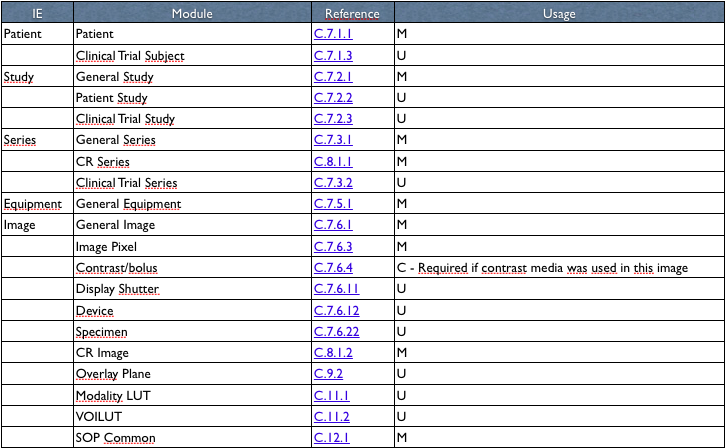
\includegraphics[width=\linewidth]{./figures/IOD-exemple.png}
}

\frame
{
	\frametitle{Objet}
	\begin{itemize}
		\item Terminologie : objet = Data Set
		\item Un Data Set est compos� de Data Elements.
		\item Chaque Data Element d�crit un attribut de l'IOD.
		\item Data Element
		\begin{itemize}
			\item �tiquette d'identification (\emph{Tag}) contenant deux num�ros.
			\item Type (\emph{VR} = \emph{Value Representation}).
			\item Taille de la valeur.
			\item Valeur.
		\end{itemize}
	\end{itemize}
}

\frame
{
	\frametitle{Objet}
	
	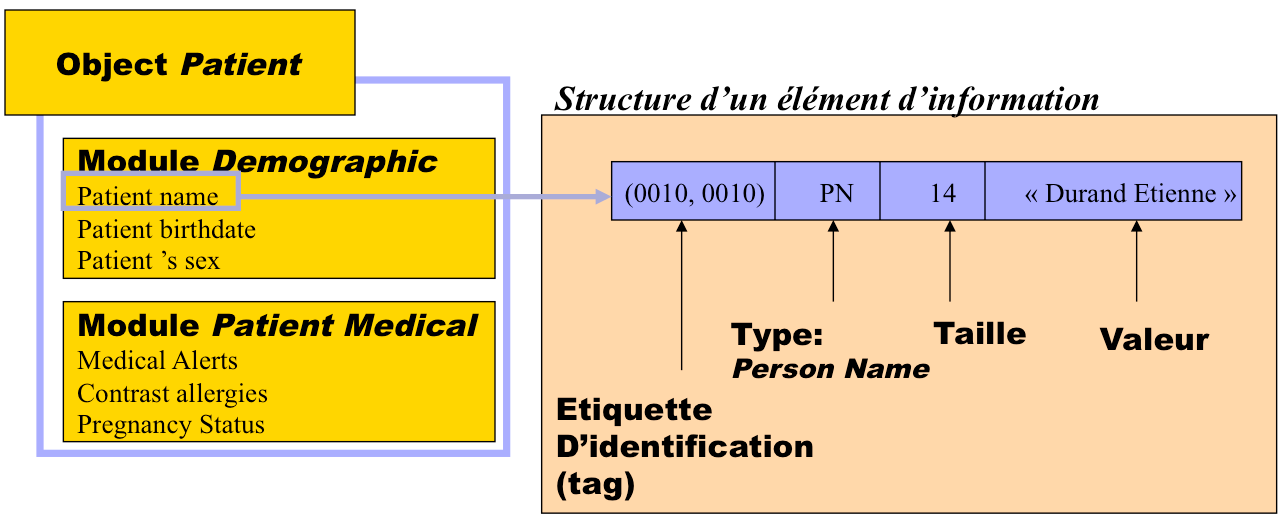
\includegraphics[width=\linewidth]{./figures/objet-dicom.png}
}

\frame
{
	\frametitle{Exemple d'objet : Examen (\emph{Study})}
	
	\begin{center}
		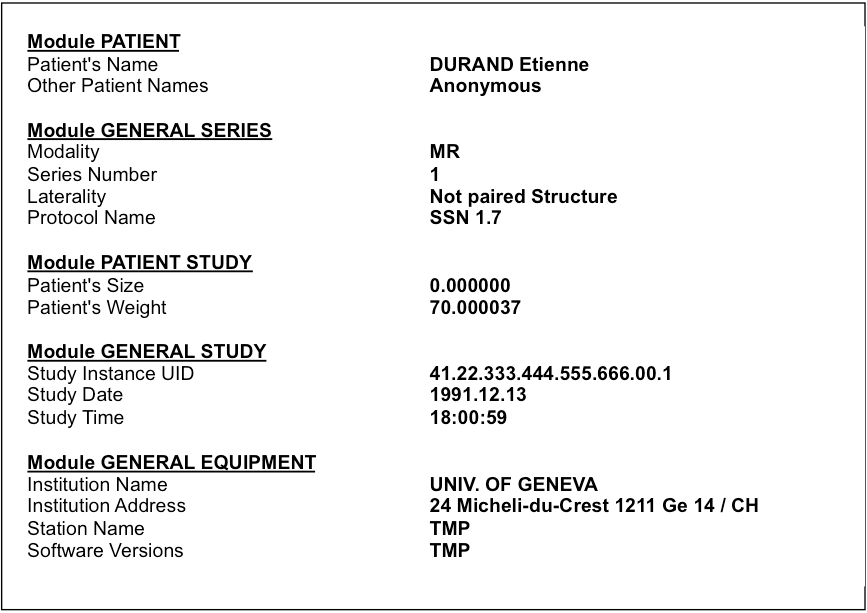
\includegraphics[width=.9\linewidth]{./figures/examen.png}
	\end{center}
}

\frame
{
	\frametitle{Exemple d'objet : Image IRM}
	
	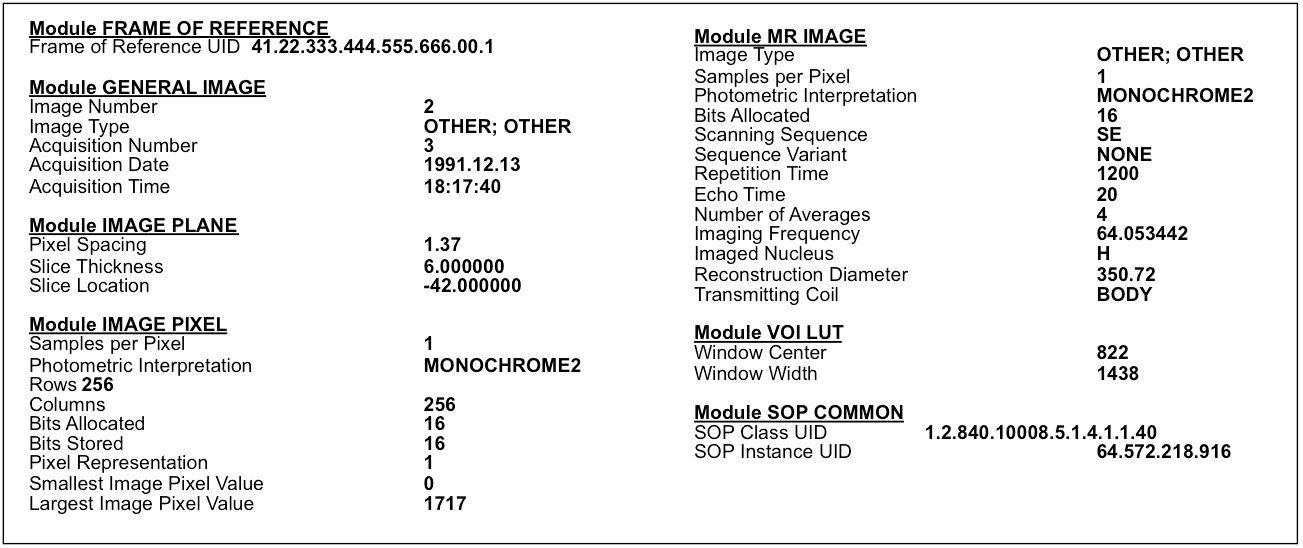
\includegraphics[width=\linewidth]{./figures/irm.png}
}

\frame
{
	\frametitle{Fichier DICOM}
	
	\begin{itemize}
		\item Encapsuler l'ensemble des objets dans un fichier.
		\begin{itemize}
			\item Ent�te : pr�-ent�te et objets.
			\item Image : donn�es brutes de l'image.
		\end{itemize}
		\item Les d�tails au prochain cours.
	\end{itemize}
}
